\documentclass[12pt]{article}
\usepackage{tikz,verbatim,pgfgantt,bm}
\usetikzlibrary{shapes,arrows}

\newcommand*\circled[1]{\tikz[baseline=(char.base)]{
            \node[shape=circle,draw,inner sep=2pt] (char) {#1};}}
            
 \begin{document}
 \thispagestyle{empty}
 \begin{figure}
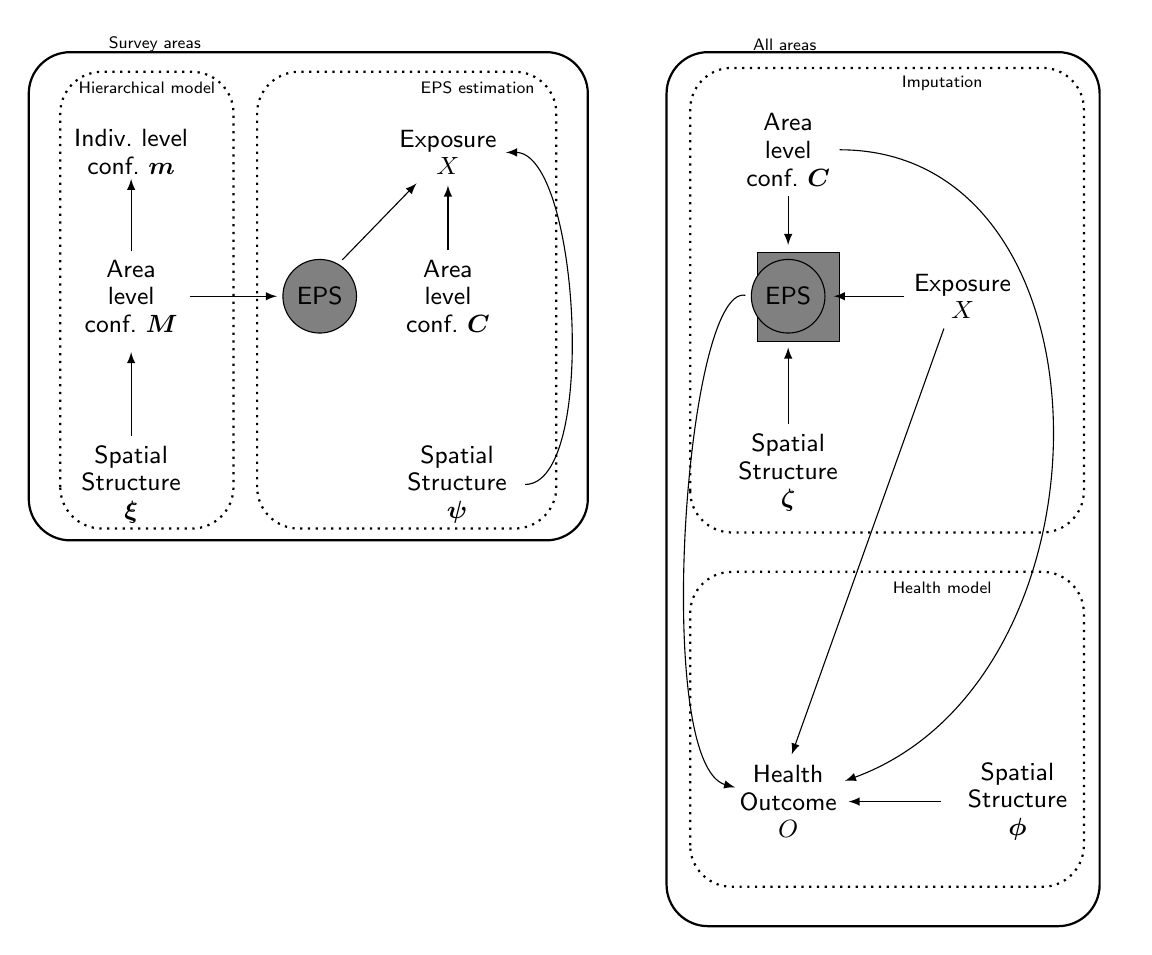
\begin{tikzpicture}
%EPS estimation
%\draw(-14,1.5) node[align=center,circle,draw=none,fill=none,font=\sffamily\fontsize{9}{10}\selectfont,minimum width=.4cm,minimum height=.4cm](2){$\mu_t$};
\draw(-15.5,1.5) node[align=center,circle,draw=none,fill=none,font=\sffamily\fontsize{9}{10}\selectfont](M){Area\\level\\conf.\ $\bm{M}$};
\node[right=1 of M, circle,align=center,draw=black, fill=gray,font=\sffamily\fontsize{9}{10}\selectfont](EPS){EPS};
\node[right=0.5 of EPS, align=center,draw=none,fill=none,font=\sffamily\fontsize{9}{10}\selectfont](C){Area\\level\\conf.\ $\bm{C}$};
\node[above=0.5 of M, align=center,font=\sffamily\fontsize{9}{10}\selectfont](m){Indiv.\ level\\ conf.\ $\bm{m}$};
\node[above=0.4 of C, align=center,circle,draw=none,fill=none,font=\sffamily\fontsize{9}{10}\selectfont](X){Exposure\\$X$};
\node[below=0.5 of M, align=center,circle,draw=none,fill=none,font=\sffamily\fontsize{9}{10}\selectfont](SS1){Spatial\\ Structure\\ $\boldsymbol{\xi}$};
\node[right=2.2 of SS1, align=center,circle,draw=none,fill=none,font=\sffamily\fontsize{9}{10}\selectfont](SS2){Spatial\\ Structure \\ $\boldsymbol{\psi$}};
%\node[below right=0.25 of SS1, align=center,circle,draw=none,fill=none,font=\sffamily\fontsize{9}{10}\selectfont](FB){Cut of \\feedback};
%\path[line](FB)()% Rounded rectangles
\draw[rounded corners=15pt,thick] (-16.8,-1.6) rectangle ++ (7.1,6.2) node[xshift=-5.5cm, yshift=0.1cm]{\fontsize{6}{7}\selectfont \sffamily Survey areas} ;
%Eq 2.1
\draw[rounded corners=15pt,dotted,thick] (-16.4,-1.45) rectangle ++ (2.2,5.8) node[xshift=-1.1cm, yshift=-0.2cm]{\fontsize{6}{7}\selectfont \sffamily Hierarchical model} ;
%Eq 2.2
\draw[rounded corners=15pt,dotted,thick] (-13.9,-1.45) rectangle ++ (3.8,5.8) node[xshift=-1cm, yshift=-0.2cm]{\fontsize{6}{7}\selectfont \sffamily EPS estimation} ;
% Arrows
\draw [->,>=latex,shorten <=-10pt, shorten >=-2pt,auto,node distance=2pt,thin] (M.north) -- (m.south);
\draw [->,>=latex,shorten >=-6pt,shorten <=-10pt,auto,node distance=2pt,thin] (SS1.north) -- (M.south);
\draw [->,>=latex,shorten >=-3pt,shorten <=-3pt,auto,node distance=2pt,thin] (SS2.0) to[out=0,in=-0,looseness=.5] (X.0);
\draw [->,>=latex,shorten >=-12pt,auto,node distance=2pt,thin] (C.north) -- (X.south);
\draw [->,>=latex,shorten >=-8pt,shorten <=2pt,auto,node distance=2pt,thin] (EPS.60) -- (X.south west);
\draw [->,>=latex,shorten >=2pt,shorten <=-5pt,auto,node distance=2pt,thin] (M.east) -- (EPS.west);
%\draw [->,>=latex,shorten >=2pt,shorten <=-5pt,auto,node distance=2pt,thin] (FB.north) -- (EPS.west);
%\draw[-,>=latex,shorten >=6pt,shorten <=-10pt,auto,node distance=2pt,thin] (FB) -- (-14.05, 1.7);
% EPS imputation
\draw[fill=gray] (-6.5,2.05) rectangle (-7.55,0.92);
\node[right=5 of EPS, align=center,circle,draw=black, fill=gray,font=\sffamily\fontsize{9}{10}\selectfont](EPS2){EPS};
\node[above=0.8 of EPS2, align=center,font=\sffamily\fontsize{9}{10}\selectfont](C2){Area\\level\\conf.\ $\bm{C}$};
\node[right=1 of EPS2, align=center,font=\sffamily\fontsize{9}{10}\selectfont](X2){Exposure\\$X$};
\node[below=0.8 of EPS2, align=center,circle,draw=none,fill=none,font=\sffamily\fontsize{9}{10}\selectfont](SS3){Spatial\\ Structure \\ $\boldsymbol{\zeta$}};
%% Arrows
\draw [->,>=latex,shorten >=5pt,shorten <=-10pt,auto,node distance=2pt,thin] (SS3.north) -- (EPS2.south);
\draw [->,>=latex,shorten >=3pt,auto,node distance=2pt,thin] (X2.west) -- (EPS2.east);
\draw [->,>=latex,shorten >=5pt,auto,node distance=2pt,thin] (C2.south) -- (EPS2.north);

% EPS adjustment
%\draw[fill=gray, dashed] (-6.2,2.15) rectangle (-7.7,0.75);
\node[below=5 of EPS2, align=center,circle,draw=none,fill=none,font=\sffamily\fontsize{9}{10}\selectfont](O){Health\\Outcome\\ $O$};
\node[right=1 of O, align=center,circle,draw=none,fill=none,font=\sffamily\fontsize{9}{10}\selectfont](SS4){Spatial\\ Structure\\ $\boldsymbol{\phi$}};
% Rounded rectangles

%% Arrows
\draw [->,>=latex,shorten >=-7pt,shorten <=2pt,auto,node distance=2pt,thin] (EPS2.west) to [out=-190,in=-195, looseness=0.35] (O);
%\draw [->,>=latex,dashed,shorten >=2pt,shorten <=-5pt,auto,node distance=.3pt,line width=.2mm] (O.west) to [out=-190,in=-190, looseness=0.42] (EPS2);
\draw [->,>=latex,shorten >=-5pt,auto,node distance=2pt,thin] (SS4.west) -- (O.east);
\draw [->,>=latex,shorten >=-5pt,auto,node distance=2pt,thin] (C2.east) to [out=0,in=20, looseness=1.15] (O);
\draw [->,>=latex,shorten >=-10pt,auto,node distance=2pt,thin] (X2.240) -- (O.80);

% Rounded rectangles
\draw[rounded corners=15pt,thick] (-8.7,-6.5) rectangle ++ (5.5,11.1) node[xshift=-4.0cm, yshift=0.1cm]{\fontsize{6}{7}\selectfont \sffamily All areas};
%Eq 2.3-2.4
\draw[rounded corners=15pt,dotted,thick] (-8.4,-1.5) rectangle ++ (5,5.9) node[xshift=-1.8cm, yshift=-0.2cm]{\fontsize{6}{7}\selectfont \sffamily Imputation} ;
%Eq 2.5
\draw[rounded corners=15pt,dotted,thick] (-8.4,-6) rectangle ++ (5,4) node[xshift=-1.8cm, yshift=-0.2cm]{\fontsize{6}{7}\selectfont \sffamily Health model} ;

\end{tikzpicture}
 \end{figure}
 \end{document}
 
 
 %%% ORIGINAL VERSION
 
\documentclass[12pt]{article}
\usepackage{tikz,verbatim,pgfgantt,bm}
\usetikzlibrary{shapes,arrows}

  \begin{figure}
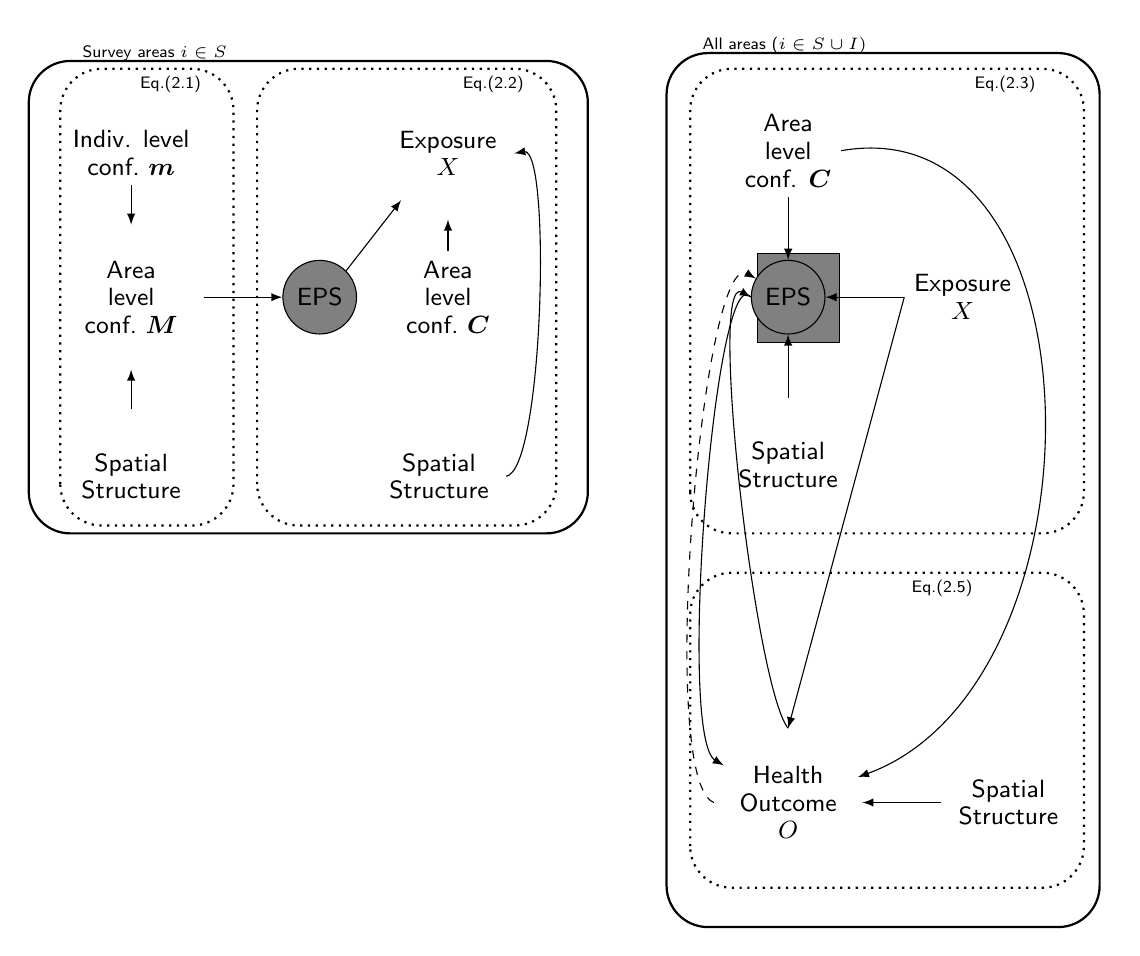
\begin{tikzpicture}
%EPS estimation
%\draw(-14,1.5) node[align=center,circle,draw=none,fill=none,font=\sffamily\fontsize{9}{10}\selectfont,minimum width=.4cm,minimum height=.4cm](2){$\mu_t$};
\draw(-15.5,1.5) node[align=center,circle,draw=none,fill=none,font=\sffamily\fontsize{9}{10}\selectfont](M){Area\\level\\conf.\ $\bm{M}$};
\node[right=1 of M, circle,align=center,draw=black, fill=gray,font=\sffamily\fontsize{9}{10}\selectfont](EPS){EPS};
\node[right=0.5 of EPS, align=center,draw=none,fill=none,font=\sffamily\fontsize{9}{10}\selectfont](C){Area\\level\\conf.\ $\bm{C}$};
\node[above=0.5 of M, align=center,font=\sffamily\fontsize{9}{10}\selectfont](m){Indiv. level\\ conf.\ $\bm{m}$};
\node[above=0.4 of C, align=center,circle,draw=none,fill=none,font=\sffamily\fontsize{9}{10}\selectfont](X){Exposure\\$X$};
\node[below=0.5 of M, align=center,circle,draw=none,fill=none,font=\sffamily\fontsize{9}{10}\selectfont](SS1){Spatial\\ Structure};
\node[right=2.2 of SS1, align=center,circle,draw=none,fill=none,font=\sffamily\fontsize{9}{10}\selectfont](SS2){Spatial\\ Structure};
% Rounded rectangles
\draw[rounded corners=15pt,thick] (-16.8,-1.5) rectangle ++ (7.1,6) node[xshift=-5.5cm, yshift=0.1cm]{\fontsize{6}{7}\selectfont \sffamily Survey areas $i \in S$} ;
%Eq 2.1
\draw[rounded corners=15pt,dotted,thick] (-16.4,-1.4) rectangle ++ (2.2,5.8) node[xshift=-0.8cm, yshift=-0.2cm]{\fontsize{6}{7}\selectfont \sffamily Eq.(2.1)} ;
%Eq 2.2
\draw[rounded corners=15pt,dotted,thick] (-13.9,-1.4) rectangle ++ (3.8,5.8) node[xshift=-0.8cm, yshift=-0.2cm]{\fontsize{6}{7}\selectfont \sffamily Eq.(2.2)} ;
% Arrows
\draw [->,>=latex,shorten >=0pt,auto,node distance=2pt,thin] (m.south) -- (M.north);
\draw [->,>=latex,shorten >=0pt,auto,node distance=2pt,thin] (SS1.north) -- (M.south);
\draw [->,>=latex,shorten >=0pt,auto,node distance=2pt,thin] (SS2.east) to[out=10,in=10, looseness=0.3] (X.east);
\draw [->,>=latex,shorten >=0pt,auto,node distance=2pt,thin] (C.north) -- (X.south);
\draw [->,>=latex,shorten >=0pt,auto,node distance=2pt,thin] (EPS.north east) -- (X.south west);
\draw [->,>=latex,shorten >=0pt,auto,node distance=2pt,thin] (M.east) -- (EPS.west);

% EPS imputation
\draw[fill=gray](-6.5,2.05) rectangle (-7.55,0.92);
\node[right=5 of EPS, align=center,circle,draw=black, fill=gray,font=\sffamily\fontsize{9}{10}\selectfont](EPS2){EPS};
\node[above=0.8 of EPS2, align=center,font=\sffamily\fontsize{9}{10}\selectfont](C2){Area\\level\\conf. $\bm{C}$};
\node[right=1 of EPS2, align=center,font=\sffamily\fontsize{9}{10}\selectfont](X2){Exposure\\$X$};
\node[below=0.8 of EPS2, align=center,circle,draw=none,fill=none,font=\sffamily\fontsize{9}{10}\selectfont](SS3){Spatial\\ Structure};
%% Arrows
\draw [->,>=latex,shorten >=0pt,auto,node distance=2pt,thin] (SS3.north) -- (EPS2.south);
\draw [->,>=latex,shorten >=0pt,auto,node distance=2pt,thin] (X2.west) -- (EPS2.east);
\draw [->,>=latex,shorten >=0pt,auto,node distance=2pt,thin] (C2.south) -- (EPS2.north);

% EPS adjustment
%\draw[fill=gray, dashed] (-6.2,2.15) rectangle (-7.7,0.75);
\node[below=5 of EPS2, align=center,circle,draw=none,fill=none,font=\sffamily\fontsize{9}{10}\selectfont](O){Health\\Outcome\\$O$};
\node[right=1 of O, align=center,circle,draw=none,fill=none,font=\sffamily\fontsize{9}{10}\selectfont](SS4){Spatial\\ Structure};
% Rounded rectangles

%% Arrows
\draw [->,>=latex,shorten >=0pt,auto,node distance=2pt,thin] (EPS2.west) to [out=-230,in=-210, looseness=0.3] (O);
\draw [->,>=latex,shorten >=0pt,auto,node distance=2pt,thin] (O.north) to [out=-230,in=-210, looseness=0.3] (EPS2.west);
\draw [->,>=latex,dashed,shorten >=0pt,auto,node distance=.3pt,thin] (O.west) to [out=-200,in=-210, looseness=0.3] (EPS2);
\draw [->,>=latex,shorten >=0pt,auto,node distance=2pt,thin] (SS4.west) -- (O.east);
\draw [->,>=latex,shorten >=0pt,auto,node distance=2pt,thin] (C2.east) to [out=10,in=20, looseness=1.1] (O);
\draw [->,>=latex,shorten >=0pt,auto,node distance=2pt,thin] (X2.west) -- (O.north);

% Rounded rectangles
\draw[rounded corners=15pt,thick] (-8.7,-6.5) rectangle ++ (5.5,11.1) node[xshift=-4.0cm, yshift=0.1cm]{\fontsize{6}{7}\selectfont \sffamily All areas ($i \in S \cup I)$};
%Eq 2.3-2.4
\draw[rounded corners=15pt,dotted,thick] (-8.4,-1.5) rectangle ++ (5,5.9) node[xshift=-1cm, yshift=-0.2cm]{\fontsize{6}{7}\selectfont \sffamily Eq.(2.3)} ;
%Eq 2.5
\draw[rounded corners=15pt,dotted,thick] (-8.4,-6) rectangle ++ (5,4) node[xshift=-1.8cm, yshift=-0.2cm]{\fontsize{6}{7}\selectfont \sffamily Eq.(2.5)} ;

\end{tikzpicture}
 \end{figure}